\documentclass[tikz,border=6pt]{standalone}
\usepackage[T1]{fontenc}
\usepackage{lmodern}
\usepackage{xcolor}

\definecolor{barblue}{HTML}{3979B9}
\definecolor{barborder}{HTML}{22527D}
\definecolor{cardred}{HTML}{C43B3B}
\definecolor{gridgray}{HTML}{D8DDE3}
\definecolor{textgray}{HTML}{3F4650}

\begin{document}
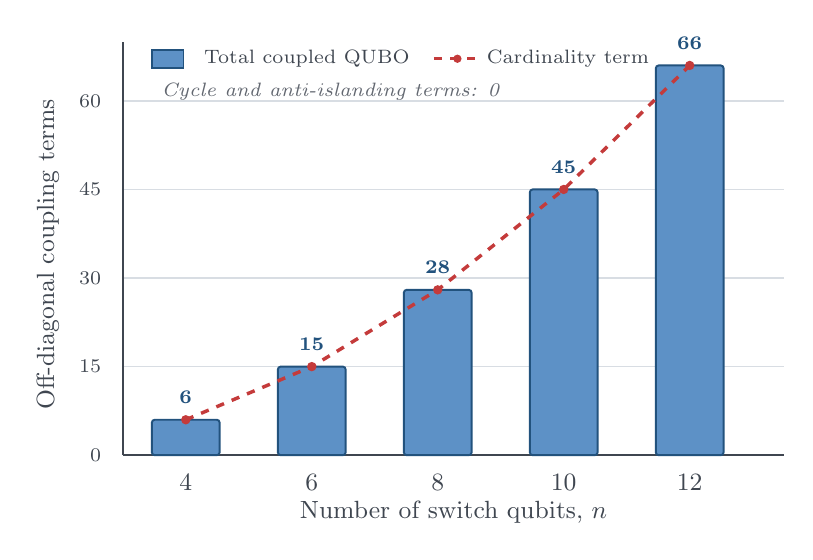
\begin{tikzpicture}[x=1cm,y=1cm,font=\sffamily]
  % Plot geometry: y scale is 0.075 cm per coupling.
  \def\ys{0.075}
  \def\xleft{1.15}
  \def\xright{9.55}
  \def\ytop{5.25}

  % Horizontal grid and y-axis labels.
  \foreach \v in {0,15,30,45,60} {
    \pgfmathsetmacro{\yy}{\v*\ys}
    \draw[gridgray,line width=0.45pt] (\xleft,\yy) -- (\xright,\yy);
    \node[anchor=east,text=textgray,font=\scriptsize] at (1.00,\yy) {\v};
  }

  % Axes.
  \draw[textgray,line width=0.8pt] (\xleft,0) -- (\xright,0);
  \draw[textgray,line width=0.8pt] (\xleft,0) -- (\xleft,\ytop);
  \node[rotate=90,text=textgray,font=\small] at (0.20,2.55)
    {Off-diagonal coupling terms};
  \node[text=textgray,font=\small] at (5.35,-0.72)
    {Number of switch qubits, $n$};

  % Bars: total coupled-QUBO terms.
  \foreach \x/\n/\v in {1.95/4/6,3.55/6/15,5.15/8/28,6.75/10/45,8.35/12/66} {
    \pgfmathsetmacro{\hh}{\v*\ys}
    \filldraw[fill=barblue!82,draw=barborder,line width=0.7pt,rounded corners=1pt]
      (\x-0.43,0) rectangle (\x+0.43,\hh);
    \node[anchor=north,text=textgray,font=\small] at (\x,-0.12) {\n};
    \node[anchor=south,text=barborder,font=\scriptsize\bfseries]
      at (\x,\hh+0.08) {\v};
  }

  % Cardinality contribution (identical to the total in this case).
  \draw[cardred,dashed,line width=1.25pt]
    (1.95,{6*\ys}) -- (3.55,{15*\ys}) -- (5.15,{28*\ys})
    -- (6.75,{45*\ys}) -- (8.35,{66*\ys});
  \foreach \x/\v in {1.95/6,3.55/15,5.15/28,6.75/45,8.35/66} {
    \fill[cardred] (\x,{\v*\ys}) circle (1.7pt);
  }

  % Compact legend and inactive-term note.
  \filldraw[fill=barblue!82,draw=barborder,line width=0.6pt]
    (1.52,4.92) rectangle (1.92,5.15);
  \node[anchor=west,text=textgray,font=\scriptsize] at (2.06,5.035)
    {Total coupled QUBO};
  \draw[cardred,dashed,line width=1.15pt] (5.10,5.035) -- (5.70,5.035);
  \fill[cardred] (5.40,5.035) circle (1.5pt);
  \node[anchor=west,text=textgray,font=\scriptsize] at (5.65,5.035)
    {Cardinality term};
  \node[anchor=west,text=textgray!82,font=\scriptsize\itshape]
    at (1.52,4.62) {Cycle and anti-islanding terms: 0};
\end{tikzpicture}
\end{document}